\renewcommand*{\arraystretch}{1.1}

\label{sec:bi-read-14}
\noindent\begin{tabularx}{\queryCardWidth}{|>{\queryPropertyCell}c|X|}
	\hline
	query & BI / 14 \\ \hline
%
	title & Top thread initiators \\ \hline
%
    pattern & \hfill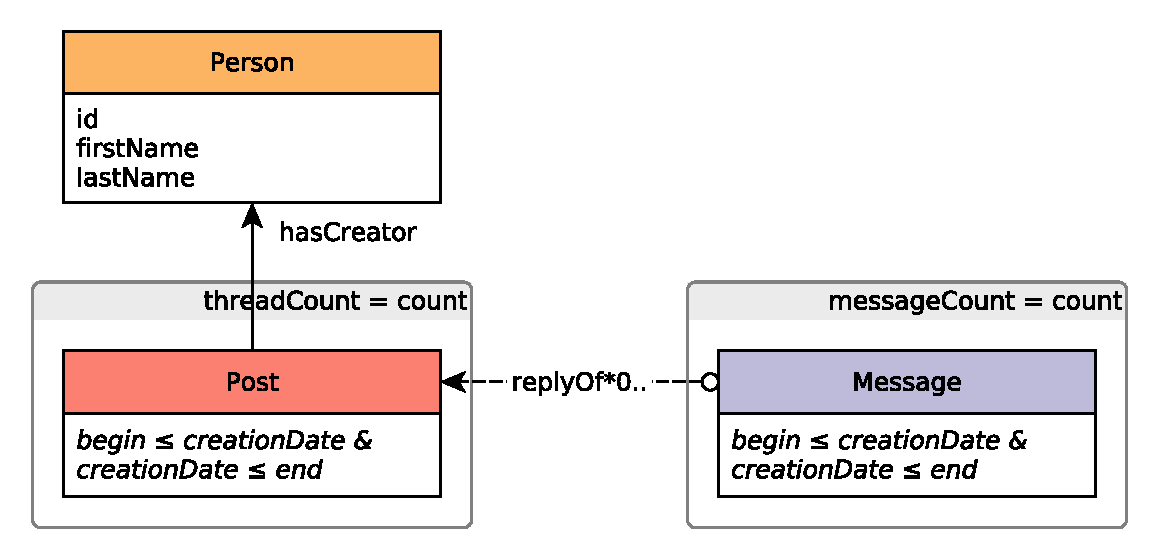
\includegraphics[scale=\patternscale,margin=0cm .2cm]{patterns/bi-read-14}\hfill\vadjust{} \\ \hline
%
	desc. & For each person, count the number Posts they created in the time
interval \texttt{(begin,\ end)}, and the number of messages in each of
their (transitive) reply trees. When calculating message counts only
consider messages created within the given time interval.

Return each person, number of Posts they created, and the count of all
messages that appeared in the reply trees (including Post at tree root)
they created.
 \\ \hline
%
	
%
	params &
	\innerCardVSpace{\begin{tabularx}{\attributeCardWidth}{|>{\paramNumberCell}c|>{\varNameCell}M|>{\typeCell}m{\typeWidth}|Y|} \hline
	\cellcolor{parameter} \color{white} \footnotesize $\mathsf{1}$ &begin& Date &  \\ \hline
	\cellcolor{parameter} \color{white} \footnotesize $\mathsf{2}$ &end& Date &  \\ \hline
	\end{tabularx}}\innerCardVSpace \\ \hline
%
	
        result &
        \innerCardVSpace{\begin{tabularx}{\attributeCardWidth}{|>{\resultNumberCell}c|>{\varNameCell}M|>{\typeCell}m{\typeWidth}|>{\resultOriginCell}c|Y|} \hline
        $\mathsf{1}$ & person.id & 64-bit Integer &R&
                 \\ \hline
        $\mathsf{2}$ & person.firstName & String &R&
                 \\ \hline
        $\mathsf{3}$ & person.lastName & String &R&
                 \\ \hline
        $\mathsf{4}$ & threadCount & 32-bit Integer &A&
                The number of threads initiated by that Person \\ \hline
        $\mathsf{5}$ & messageCount & 32-bit Integer &A&
                The number of messages created in all the threads this Person initiated \\ \hline
        \end{tabularx}}\innerCardVSpace \\ \hline
	
%
	sort        &
        \innerCardVSpace{\begin{tabular}{|>{\sortNumberCell}c|>{\varNameCell}l|>{\directionCell}c|} \hline
        $\mathsf{1}$ & messageCount & $\desc$ \\ \hline
        $\mathsf{2}$ & person.id & $\asc$ \\ \hline
        \end{tabular}}\innerCardVSpace \\ \hline
	%
	limit & 100 \\ \hline
	%
	CPs &
	\multicolumn{1}{>{\raggedright}l|}{
	    \chokePoint{1.2}, 
	    \chokePoint{2.2}, 
	    \chokePoint{2.3}, 
	    \chokePoint{3.2}, 
	    \chokePoint{7.2}, 
	    \chokePoint{7.3}, 
	    \chokePoint{7.4}
	    } \\ \hline
	%
    %
\end{tabularx}
\queryCardVSpace